\documentclass[letterpaper]{l3doc}

\usepackage[mono = false]{libertine}
\usepackage{geometry,pdfpages,tikz,xfrac,hologo,authblk}
\hologoFontSetup{general = \sffamily}
\newenvironment{example}{\begin{list}{}{\leftmargin=\parindent}\item }{\end{list}}
\fvset{xleftmargin = \parindent}
\usepackage[fontset = none]{ctex}
\setCJKmainfont[AutoFakeBold = 4, AutoFakeSlant]{LXGW WenKai}
\setCJKsansfont[AutoFakeBold = 4, AutoFakeSlant]{LXGW WenKai}
\setCJKmonofont[AutoFakeBold = 4, AutoFakeSlant]{LXGW WenKai}
\usepackage[os = mac]{menukeys}

\title
{
  \cls{litetable} 文档类:多彩的课程表
  \thanks{\url{https://github.com/xiamyphys/litetable}}
}

\author{夏明宇,香港中文大学(深圳)}

\affil{\href{mailto:xiamyphys@gmail.com}{xiamyphys@gmail.com}}

\date{Version 3.1A, \today}

\begin{document}

\maketitle

\begin{abstract}
  本文档为 \cls{litetable} 文档类的用户手册. 该文档类提供了一个多彩的课程表设计. 欢迎通过邮件 \href{mailto:xiamyphys@gmail.com}{xiamyphys@gmail.com} 或 \href{https://github.com/xiamyphys/litetable/issues}{GitHub} 提供建议或反馈bug. 本手册提供英文、\textbf{中文}和粤语版本.
\end{abstract}

\section{介绍}

\subsection{所需宏包}

该文档类基于 \cls{article} 文档类. 它由 \hologo{LaTeX3} 构建,并需要 \pkg{tikz} 宏包. 

\subsection{兼容性}

所用的测试平台为 macOS 15.1 / Overleaf / Ubuntu 22.04.2,兼容 \hologo{TeX}Live 2021 -- 2024发行版,在 \hologo{pdfLaTeX} 和 \hologo{XeLaTeX} 编译器下均可正常运行.

\section{使用}

\subsection{载入 \cls{litetable} 并生成课程表框架}

同加载其他文档类一样,只需写下

\begin{Verbatim}
  \documentclass{litetable}
\end{Verbatim}

接下来的命令需要带有 \cmd{remember picture, overaly} 选项的 \cmd{tikzpicture} 环境.

\subsubsection{命令:\cs{maketable}}

\begin{example}
  \cs{maketable}\oarg{semester}\marg{title}\qquad
  \cs{maketable}\marg{title}\oarg{semester}
\end{example}

此命令有两个参数,可生成一个空白的课程表框架. 可选参数可在页面的右上角添加学期块,强制参数可指定标题.

\subsubsection{命令:\cs{more}}

\begin{example}
  \cs{more}\marg{comment}
\end{example}

此命令可在页面的右下角添加备注.

\subsubsection{命令:\cs{timelist}}

\begin{example}
  \cs{timelist}\oarg{rows}\marg{time list}\qquad
  \cs{timelist}\marg{time list}\oarg{rows}
\end{example}

此命令有两个参数,可选参数可直接决定课程表的行数,强制参数可在课程表的左侧添加时间列表. 输入数组的用例如下

\begin{Verbatim}
  \timelist[13]
  {
    08:05 -> 08:50, 08:55 -> 09:40, 10:00 -> 10:45, 10:50 -> 11:35,
    11:40 -> 12:25, 13:30 -> 14:15, 14:20 -> 15:05, 15:15 -> 16:00,
    16:05 -> 16:50, 18:30 -> 19:15, 19:20 -> 20:05, 20:10 -> 20:55
  }
\end{Verbatim}

对于两个参数的不同使用情况,\cls{litetable} 会以如下规则生成对应行数的课程表框架.

\begin{itemize}
  \item 若强制参数接收了$X$组时间,可选参数接收的值为$X+a$,则课程表的左侧只有$1 \sim X$行会显示时间,后面几行不显示时间.
  \item 若强制参数接收了$X+a$组时间,可选参数接收的值为$X$, 则会生成只有$X$行的课程表,多余的时间组将被忽略,并返回一个警告.
  \item 如果只想在课程表左侧添加一列序号,使强制变量为空即可.
\end{itemize}

\subsubsection{命令:\cs{weeklist}}

\begin{example}
  \cs{weeklist}\oarg{default weeks}\marg{week list}\qquad
  \cs{weeklist}\marg{week list}\oarg{default weeks}
\end{example}

此命令有两个参数. 第一个可选参数可决定默认的星期数并会在每个课程块的右下角显示,第二个强制参数可在课程表的顶部添加对应宽度比例的工作日. 输入列表的第一行为工作日格式,第二行为对应的宽度比例,两行之间用分号 (;) 分隔. 例如

\begin{Verbatim}
  \weeklist[Weeks 1 - 16]{Mon -> 4, Tue -> 5, Wed -> 4, Thu -> 6, Fri -> 5}
\end{Verbatim}

\begin{figure}[htbp]
  \centering
  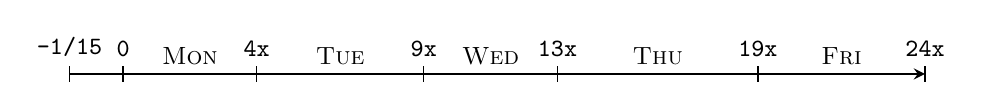
\begin{tikzpicture}[every node/.style={font=\small\sffamily\scshape}]
    \draw [thick,->,>=stealth] (-.84\linewidth/15,0) -- (.84\linewidth,0);
    \draw (-.84\linewidth/15,-.1) --++ (0,.2) node [above] {\verb|-1/15|};
    \draw (0,-.1) --++ (0,.2) node [above] {\verb|0|};
    \draw (4*.84\linewidth/24,-.1) --++ (0,.2) node [above] {\verb|4x|};
    \draw (9*.84\linewidth/24,-.1) --++ (0,.2) node [above] {\verb|9x|};
    \draw (13*.84\linewidth/24,-.1) --++ (0,.2) node [above] {\verb|13x|};
    \draw (19*.84\linewidth/24,-.1) --++ (0,.2) node [above] {\verb|19x|};
    \draw (.84\linewidth,-.1) --++ (0,.2) node [above] {\verb|24x|};
    \node [above] at (2*.84\linewidth/24,0) {Mon};
    \node [above] at (6.5*.84\linewidth/24,0) {Tue};
    \node [above] at (11*.84\linewidth/24,0) {Wed};
    \node [above] at (16*.84\linewidth/24,0) {Thu};
    \node [above] at (21.5*.84\linewidth/24,0) {Fri};
  \end{tikzpicture}
\end{figure}

此时 \cs{course} 命令中键 \keys{weeks} 的默认值被赋为 \cmd{Weeks 1 - 16}. 如果输入的工作日的数量比输入的宽度比例数量多,则多余的工作日将被忽略并返回一条警告.

\subsection{添加课程块}

使用 \cs{course} 命令在当前工作日添加课程块. 此命令有两个参数.

\begin{example}
  \cs{course}\oarg{keyvals}\marg{class start number}\marg{class end number}
\end{example}

第一个可选参数接收下列键:\keys{color} \keys{subject} \keys{location} \keys{teacher} \keys{weeks}. 键 \keys{color} 的默认值为 \cmd{DarkSlateGray},键 \keys{weeks} 的默认值由命令 \cs{weeklist} 的第一个参数决定. 第二个和第三个强制参数分别为课程的开始和结束序号. \cs{course} 命令的用例如下

\begin{Verbatim}
  \course [ color = DarkSlateGray, subject = litetable,
            location = Hong Kong, teacher = M.Y. Xia
          ] {8} {8}
\end{Verbatim}

\begin{center}
  \noindent\fbox
  {
    \parbox{.96\linewidth}
    {
      将此课程块的颜色设置为 \cmd{DarkSlateGray},此课程名称为 \cmd{litetable},上课地点为 \cmd{Hong Kong},教师为 \cmd{M.Y. Xia},在当日的第 \cmd{8} 节课开始,第 \cmd{8} 节课结束.
    }
  }
\end{center}

\begin{itemize}
  \item 可通过 \cs{newday} 命令切换到下一个工作日.
  \item 若课程块的高度只有一个单位,即$\marg{class start number} = \marg{class end number}$,则键 \keys{location} 和 \keys{teacher} 的值将输出在同一行并以逗号 (,) 间隔,键 \cmd{weeks} 的值将不会输出.
  \item 若键 \keys{location} 和 \keys{teacher} 均未赋值,则键 \keys{subject} 的值将输出在课程块的中心.
\end{itemize}

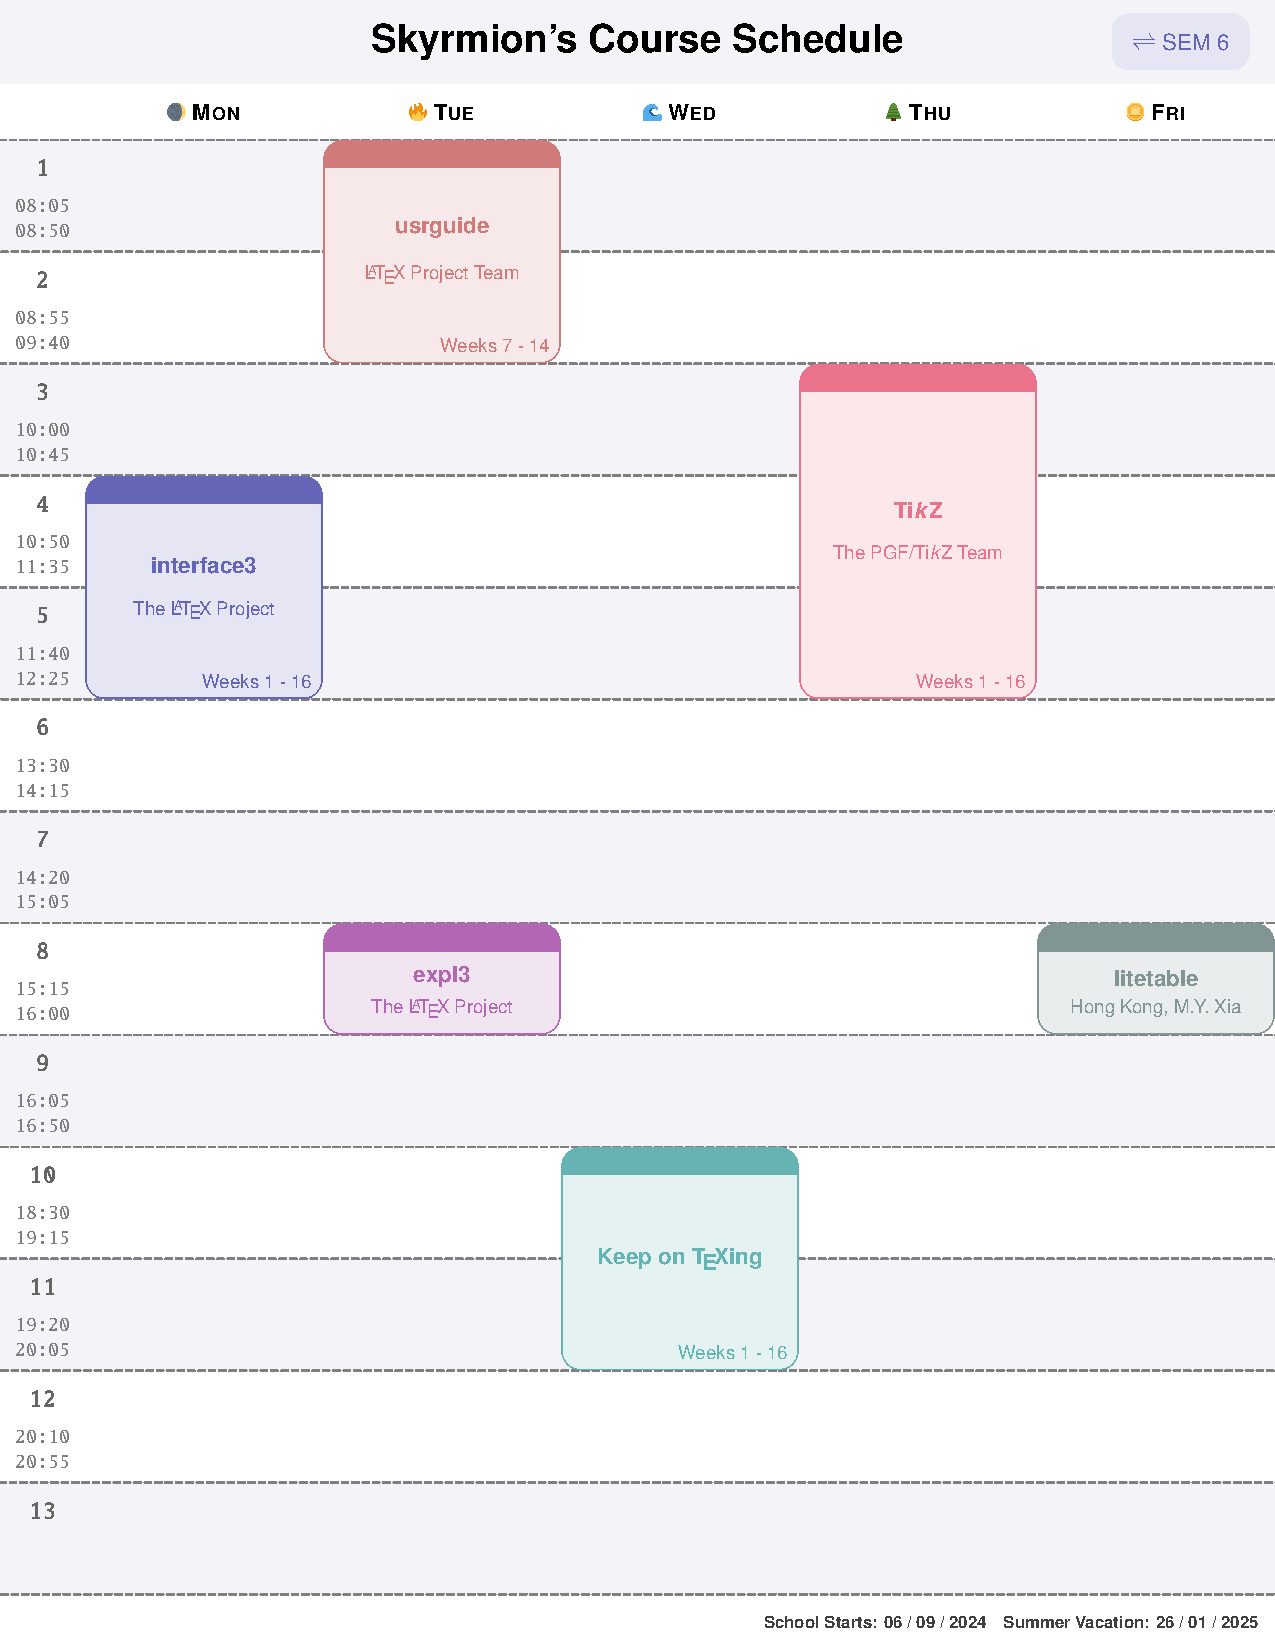
\includepdf[pages = 1]{litetable-demo.pdf}

\end{document}